\chapter{Multivariate models}\label{chap7}

We describe how to perform Bayesian inference in multivariate response models: multivariate regression, seemingly unrelated regression, instrumental variables, and multivariate probit model. In particular, we show the posterior distributions of the parameters, and perform some applications and simulations. Again, we show how to perform inference in these models using three levels of programming skills: GUI, packages, and programming from scratch the algorithms. Finally, there are some mathematical and computational exercises.

Remember that we can run our GUI typing

\begin{tcolorbox}[enhanced,width=4.67in,center upper,
	fontupper=\large\bfseries,drop shadow southwest,sharp corners]
	\textit{R code. How to display our graphical user interface}
	\begin{VF}
		\begin{lstlisting}[language=R]
	shiny::runGitHub("besmarter/BSTApp", launch.browser = T)
\end{lstlisting}
	\end{VF}
\end{tcolorbox} 

in the \textbf{R} package console or any \textbf{R} code editor.

\section{Multivariate regression}\label{sec71}

A complete presentation of this model is given in Section \ref{sec44}. We show here the setting, and the posterior distributions for facility in exposition. In particular, there are $M$ multiply dependent variables which share the same set of regressors, and their stochastic errors are contemporaneously correlated. In particular, $\bm{Y}=\left[{\bf{y_{1}}},{\bf{y_{2}}},\ldots,{\bf{y_{M}}}\right]$ is an $ N\times M$ matrix that is generated by $\bm{Y}=\bm{X}\bm{B}+\bm{U}$ where $\bm{X}$ is an $ N\times K$ matrix of regressors, $\bm{B}=\left[\bm{\beta}_{1} \ \bm{\beta}_{2} \ldots \bm{\beta}_{M}\right]$ is a $ K\times M$ matrix of parameters, and $\bm{U}=\left[\bm{\mu}_{1} \ \bm{\mu}_{2}\ldots \bm{\mu}_{M}\right]$ is a matrix of stochastic random errors such that $\bm{\mu}_i\sim{N}(\bm{0},\bm{\Sigma})$, $i=1,2,\dots,N$ is each row of $\bm{U}$.

The prior is given by   $\pi(\bm{B}|\bm{\Sigma})\sim{N}(\bm{B}_0,\bm{V}_0, \bm{\Sigma})$ and $\pi(\bm{\Sigma})\sim{I}{W}(\bm{\Psi}_0,\alpha_0)$. Therefore, the conditional posterior distributions are
\begin{equation*}
	\bm{B}|\bm{\Sigma}, \bm{Y}, \bm{X} \sim{N}(\bm{B}_n, \bm{V}_n, \bm{\Sigma}), 
\end{equation*}
\begin{equation*}
	\bm{\Sigma}| \bm{Y}, \bm{X} \sim {I}{W}(\bm{\Psi}_n, \alpha_n),
\end{equation*}

where $\bm{V}_n=(\bm{X}^{\top}\bm{X}+\bm{V}_0^{-1})^{-1}$, $\bm{B}_n=\bm{V}_n(\bm{V}_0^{-1}\bm{B}_0 + \bm{X}^{\top}\bm{X}\hat{\bm{B}})$, $\hat{\bm{B}}=(\bm{X}^{\top}\bm{X})^{-1}\bm{X}^{\top}\bm{Y}$, $\bm{\Psi}_n = {\bf{\Psi}}_{0}+{\bf{S}}+{\bf{B}}_{0}^{\top}{\bf{V}}_{0}^{-1}{\bf{B}}_{0}+\widehat{\bf{B}}^{\top}{\bf{X}}^{\top}{\bf{X}}\widehat{\bf{B}}-{\bf{B}}_n^{\top}{\bf{V}}_n^{-1}{\bf{B}}_n$, and $\alpha_n = \alpha_0 + N$. We can use a Gibbs sampling algorithm in this model since the conditional posterior distributions are standard.\\

\textbf{Example: The effect of institutions on per capita gross domestic product}

To illustrate multivariate regression models, we used the dataset provided by \cite{Acemoglu2001}, who analyzed the effect of property rights on economic growth.

Let's assume that the point of departure is the following \textit{simultaneous structural} economic model:\footnote{This is a model that captures the potential underlying economic relationship between the variables.}
\begin{align}\label{eq:str1}
	\log(\text{pcGDP95}_i)=\beta_1+\beta_2\text{PAER}_i+\beta_3 \text{Africa}+\beta_4 \text{Asia}+\beta_5 \text{Other}+u_{1i},
\end{align}
\begin{align}\label{eq:str2}
	\text{PAER}_i=\alpha_1+\alpha_2\log(\text{pcGDP95}_i)+\alpha_3\log(\text{Mort}_i)+u_{2i},
\end{align}
where \textit{pcGDP95}, \textit{PAER} and \textit{Mort} are the per capita gross domestic product (GDP) in 1995, the average index of protection against expropriation between 1985 and 1995, and the settler mortality rate during the time of colonization, respectively. \textit{Africa}, \textit{Asia} and \textit{Other} are dummies for continents, with \textit{America} as the baseline group.

In this model, there is \textit{reverse (simultaneous) causality} due to the contemporaneous effect of \textit{GDP} on \textit{PAER}, and vice verse.\footnote{\textit{Simultaneous causality} is the most controversial causation issue from a philosophy of science perspective. The root of the issue is that causation is typically based on the time sequence of cause and effect.} Therefore, estimation of the Equations \ref{eq:str1} and \ref{eq:str2} without taking into account this phenomenon generates posterior mean estimates that are \textit{biased} and \textit{inconsistent} from a sampling (frequentist) point of view.\footnote{Observe that $\mathbb{E}[u_1\text{PAER}]\neq 0$, which means failing to meet a necessary requirement to get \textit{unbiased} and \textit{consistent} estimators of $\bm{\beta}$. See exercise 1.} A potential strategy to tackle this issue is to estimate the \textit{reduced-form} model, that is, a model without \textit{simultaneous causality} where all \textit{endogenous variables} are function of \textit{exogenous variables}. The former variables are determined within the model ($\log(\text{pcGDP95}_i)$ and PAER in this example), and the latter are determined outside the model ($\log(\text{Mort}_i)$, Africa, Asia, and Other in this example).

Replacing Equation \ref{eq:str2} into Equation \ref{eq:str1}, and solving for $\log(\textit{pcGDP95})$,
\begin{align}\label{eq:red1}
	\log(\text{pcGDP95}_i)=\pi_1+\pi_2\log(\text{Mort}_i)+\pi_3 \text{Africa}+\pi_4 \text{Asia}+\pi_5 \text{Other}+e_{1i}.   
\end{align}
Then, replacing Equation \ref{eq:red1} into Equation \ref{eq:str2}, and solving for \textit{PAER},
\begin{align}\label{eq:red2}
	\text{PAER}_i=\gamma_1+\gamma_2\log(\text{Mort}_i)+\gamma_3 \text{Africa}+\gamma_4 \text{Asia}+\gamma_5 \text{Other}+e_{2i},
\end{align}
where $\pi_2=\frac{\beta_2\alpha_3}{1-\beta_2\alpha_2}$ and $\gamma_2=\frac{\alpha_3}{1-\beta_2\alpha_2}$ given $\beta_2\alpha_2\neq 1$, that is, independent equations (see Exercise 2). 

Observe that equations \ref{eq:red1} and \ref{eq:red2} have the form of a multivariate regression model where the common set of regressors is $\bm{X}=\left[\log(\textbf{Mort}) \ \textbf{Africa} \ \textbf{Asia} \ \textbf{Other}\right]$ and $\bm{Y}=\left[\log(\textbf{pcGDP95}) \ \textbf{PAER}\right]$. Thus, we can estimate this model using the setup of this section.

Thus, we estimate in a first stage the parameters from the \textit{reduced-form} model (Equations \ref{eq:red1} and \ref{eq:red2}), but the main interest is the parameters of the \textit{structural} model (Equations \ref{eq:str1} and \ref{eq:str2}). Thus, a valid question is if we can recover the \textit{structural} parameters from the \textit{reduced-form} parameters. There are two criteria to respond this question: the order condition, which is necessary, and the rank condition, which is necessary and sufficient.\\
 
\textit{The order condition}

Given a system of equations with $M$ endogenous variables, and $K$ exogenous variables (including the intercept), there are two ways to assess the order condition:
\begin{itemize}
	\item The parameters of an equation in the system are identified if there are at least $M-1$ variables excluded from the equation (\textit{exclusion restrictions}). The equation is \textit{exactly identified} if the number of excluded variables is $M-1$, and is \textit{over identified} if the number of excluded variables is greater than $M-1$.
	\item The parameters of equation $m$ in the system are identified if $K-K_m\geq M_m-1$, where $K_m$ and $M_m$ are the number of exogenous and endogenous variables in equation $m$, respectively. The $m$-th equation is \textit{exactly identified} if $K-K_m = M_m-1$, and \textit{over identified} if if $K-K_m > M_m-1$. 
\end{itemize}

We can see from Equations \ref{eq:str1} and \ref{eq:str2} in this example that $K=5$, $M=2$, $K_1=4$, $K_2=2$, $M_1=2$ and $M_2=2$. This means that $K-K_1=1=M-1$ and $K-K_2=3>M-1=1$, that is, the order condition says that both equations satisfy the necessary condition of identification, the first equation would be \textit{exactly identified}, and the second equation would be \textit{over identified}. Observe that there is one excluded variable from the first equation, and there are three excluded variables from the second equation.
\\

\textit{The rank condition}

The rank condition (necessary and sufficient) says that given a \textit{structural} model with $M$ equations ($M$ endogenous variables), an equation is identified if and only if there is at least one determinant different from zero from a $(M-1)\times(M-1)$ matrix built using the excluded variables in the analyzed equation, but included in any other equation of the system.

It is useful to build the \textit{identification matrix} to implement the \textit{rank} condition. Table \ref{tab:71} shows this matrix in this example.

\begin{table}[!h]
	%\noautomaticrules
	\tabletitle{Identification matrix.}\label{tab:71}%
	\begin{tabular}{ccccccc}
		$\log(\text{pcGDP95})$ & PAER & Constant & $\log(\text{Mort})$ & Africa & Asia & Other \\
		\hline
		1 & -$\beta_2$ & -$\beta_1$ & 0 & -$\beta_3$ & -$\beta_4$ & -$\beta_5$\\
		-$\alpha_2$ & 1 & $-\alpha_1$ & -$\alpha_3$ & 0 & 0 & 0 \\
	\end{tabular}
\end{table}

The only excluded variable in the $\log(\text{pcGDP95})$ equation is $\log(\text{Mort})$. Then, there is just one matrix that can be built using the excluded variables from this equation $[-\alpha_3]$ (see column 4 in Table \ref{tab:71}). Thus, the determinant of this matrix is $-\alpha_3$, and as far as this coefficient is different to zero, that is, that the mortality rate is relevant in the $PAER$ equation ($\alpha_3\neq 0$), the coefficients in $\log(\text{pcGDP95})$ equation are \textit{exactly identified}. For instance, $\beta_2=\frac{\pi_2}{\gamma_2}$, which is the effect of property rights on GDP, is exactly identified. 

Observe the importance of excluding $\log(\text{Mort})$ from the $\log(\text{pcGDP95})$ equation, but including $\log(\text{Mort})$ in the PAER equation. This is called \textit{exclusion restriction}, and it is the requirement of having an exogenous source of variability in the PAER equation that helps to identify the $\log(\text{pcGDP95})$ equation. Having relevant exogenous sources of variability is a very important aspect in identification, estimation and inference of \textit{structural} parameters.

Regarding the identification of the \textit{structural} parameters in the PAER equation, there are three potential matrices that can be constructed: $[-\beta_3]$, $[-\beta_4]$ and $[-\beta_5]$ (see columns 5, 6 and 7 in Table \ref{tab:71}), as far as any of these parameters are relevant in the $\log(\text{pcGDP95})$ equation, we achieve identification of the PAER equation. In this case, this equation is \textit{over identified}, that is, there are many ways to find the parameters in this equations. For instance, $\alpha_2=\gamma_3/\pi_3=\gamma_4/\pi_4=\gamma_5/\pi_5$ (see Exercise 2).

In general, trying to recover the \textit{structural} parameters from the \textit{reduced-form} parameters can be challenging due to the requirement of relevant identification restrictions that can be hard to find in some applications.\footnote{Good text books at introductory level for identification in linear systems are \cite[Chap. ~19]{gujarati2009basic} and \cite[Chap. ~16]{wooldridge2016introductory}.}

We set non-informative priors in this example, $\bm{B}_0=\left[\bm{0}_5 \ \bm{0}_5\right]$, $\bm{V}_0=100\bm{I}_K$, $\bm{\Psi}_0=5\bm{I}_2$ and $\alpha_0=5$.\footnote{Observe that we are setting the priors in the \textit{reduced-form} model; this may have unintended consequences for the posterior distributions of the \textit{structural} parameters, which are ultimately the parameters researchers are interested in. See \cite[p.~302]{koop2003bayesian} for good references in this topic.} Once our GUI is displayed (see beginning of this chapter), we should follow Algorithm \ref{alg:MultReg} to run multivariate linear models in our GUI (see Chapter \ref{chapGUI} for details, particularly how to set the data set):
\begin{algorithm}[h!]
	\caption{Multivariate linear model}\label{alg:MultReg}
	\begin{algorithmic}[1]  		 			
		\State Select \textit{Multivariate Models} on the top panel
		\State Select \textit{Simple Multivariate} model using the left radio button
		\State Upload the dataset selecting first if there is header in the file, and the kind of separator in the \textit{csv} file of the dataset (comma, semicolon, or tab). Then, use the \textit{Browse} button under the \textbf{Choose File} legend
		\State Select MCMC iterations, burn-in and thinning parameters using the \textit{Range sliders}
		\State Select the number of dependent variables in the box \textbf{Number of endogenous variables: m}
		\State Select the number of independent variables (including the intercept) in the box \textbf{Number of exogenous variables: k}
		\State Set the hyperparameters: mean vectors, covariance matrix, degrees of freedom, and the scale matrix. This step is not necessary as by default our GUI uses non-informative priors
		\State Click the \textit{Go!} button
		\State Analyze results
		\State Download posterior chains and diagnostic plots using the \textit{Download Posterior Chains} and \textit{Download Posterior Graphs} buttons
	\end{algorithmic} 
\end{algorithm}

The following \textbf{R} code shows how to perform the Gibss sampling algorithm in this example using the dataset \textit{4Institutions.csv}. We ask to run this example using the \textit{rmultireg} command from the \textit{bayesm} package as an exercise. We find that the posterior mean \textit{structural} effect of property rights on GDP is 0.98, and the 95\% credible interval is (0.56, 2.87). This means that there is evidence supporting a positive effect of property rights on gross domestic product. 

\begin{tcolorbox}[enhanced,width=4.67in,center upper,
	fontupper=\large\bfseries,drop shadow southwest,sharp corners]
	\textit{R code. The effect of institutions on per capita GDP}
	\begin{VF}
		\begin{lstlisting}[language=R]
rm(list = ls())
set.seed(12345)
DataInst <- read.csv("DataApplications/4Institutions.csv", sep = ",", header = TRUE, fileEncoding = "latin1")
attach(DataInst)
Y <- cbind(logpcGDP95, PAER)
X <- cbind(1, logMort, Africa, Asia, Other)
M <- dim(Y)[2]
K <- dim(X)[2]
N <- dim(Y)[1]
# Hyperparameters
B0 <- matrix(0, K, M)
c0 <- 100
V0 <- c0*diag(K)
Psi0 <- 5*diag(M)
a0 <- 5
# Posterior parameters
Bhat <- solve(t(X)%*%X)%*%t(X)%*%Y 
S <- t(Y - X%*%Bhat)%*%(Y - X%*%Bhat)
Vn <- solve(solve(V0) + t(X)%*%X) 
Bn <- Vn%*%(solve(V0)%*%B0 + t(X)%*%X%*%Bhat)
Psin <- Psi0 + S + t(B0)%*%solve(V0)%*%B0 + t(Bhat)%*%t(X)%*%X%*%Bhat - t(Bn)%*%solve(Vn)%*%Bn
an <- a0 + N
#Posterior draws
s <- 10000 #Number of posterior draws
SIGs <- replicate(s, LaplacesDemon::rinvwishart(an, Psin))
BsCond <- sapply(1:s, function(s) {MixMatrix::rmatrixnorm(n = 1, mean=Bn, U = Vn,V = SIGs[,,s])})
summary(coda::mcmc(t(BsCond)))
SIGMs <- t(sapply(1:s, function(l) {gdata::lowerTriangle(SIGs[,,l], diag=TRUE, byrow=FALSE)}))
summary(coda::mcmc(SIGMs))
hdiBs <- HDInterval::hdi(t(BsCond), credMass = 0.95) # Highest posterior density credible interval
hdiBs
hdiSIG <- HDInterval::hdi(SIGMs, credMass = 0.95) # Highest posterior density credible interval
hdiSIG
beta2 <- BsCond[2,]/BsCond[7,] 
summary(coda::mcmc(beta1)) # Effect of property rights on GDP
Iterations = 1:10000
Thinning interval = 1 
Number of chains = 1 
Sample size per chain = 10000 
1. Empirical mean and standard deviation for each variable,
plus standard error of the mean:
Mean             SD       Naive SE Time-series SE 
0.9796        16.8430         0.1684         0.1684 
2. Quantiles for each variable:
2.5%    25%    50%    75%  97.5% 
0.5604 0.7984 0.9677 1.2329 2.8709 
\end{lstlisting}
	\end{VF}
\end{tcolorbox} 

\section{Seemingly unrelated regression}\label{sec72}

In seemingly unrelated regression (SUR) models there are $M$ dependent variables with potentially different regressors such that the stochastic errors are contemporaneously correlated. This is $\bm{y}_{j}=\bm{X}_{j}\bm{\beta}_j+\bm{\mu}_{j}$, where $\bm{y}_j$ is a $N$-dimensional vector, $\bm{X}_j$ is a matrix of dimension $N\times K_m$ of regressors, $\bm{\beta}_j$ is a $K_m$-dimensional vector of location parameters, and $\bm{\mu}_j$ is a $N$-dimensional vector of stochastic errors, $m=1,2,\dots,M$.
	
Setting $\bm{\mu}_i=\left[\mu_{i1} \ \mu_{i2} \dots \mu_{iM}\right]^{\top}$ such that $\bm{\mu}_i\sim{N}(\bm{0},\bm{\Sigma})$, and stacking the $M$ equations, we can write $\bm{y}=\bm{X}\bm{\beta}+\bm{\mu}$ where $\bm{y}=\left[\bm{y}_{1}^{\top} \ \bm{y}_{2}^{\top} \dots \bm{y}_{M}^{\top}\right]^{\top}$ is a $MN$-dimensional vector,  $\bm{\beta}=\left[\bm{\beta}_{1}^{\top} \ \bm{\beta}_{2}^{\top} \ldots \bm{\beta}_{M}^{\top}\right]^{\top}$ is a $ K$ dimensional vector, $K=\sum_{m=1}^{M} K_m$, $\bm{X}$ is an $MN\times K$ block diagonal matrix composed of $\bm{X}_{m}$ and $\bm{\mu}=\left[\bm{\mu}_{1}^{\top} \ \bm{\mu}_{2}^{\top} \dots ,\bm{\mu}_{M}^{\top}\right]^{\top}$ is a $MN$-dimensional vector of stochastic errors such that $\bm{\mu}\sim{N}(\bm{0},\bm{\Sigma}\otimes \bm{I}_N)$.
Then, 
\begin{align*}
	p(\bm{\beta},\bm{\Sigma}|\bm{y},\bm{X})\propto \left|\bm{\Sigma} \right|^{-N/2}\exp\left\{ -\frac{1}{2}(\bm{y}-\bm{X\beta})^{\top}(\bm{\Sigma}^{-1}\otimes \bm{I}_N\})(\bm{y}-\bm{X\beta})\right\}.
\end{align*}

Using independent priors $\pi(\bm{\beta})\sim{N}(\bm{\beta}_0,\bm{B}_0)$ and $\pi(\bm{\Sigma}^{-1})\sim{W}(\alpha_0,\bm{\Psi}_0)$, the posterior distributions are
\begin{equation*}
	\bm{\beta}|\bm{\Sigma}, \bm{y}, \bm{X} \sim {N}(\bm{\beta}_n, \bm{B}_n), 
\end{equation*}
\begin{equation*}
	\bm{\Sigma}^{-1}|\bm{\beta}, \bm{y}, \bm{X} \sim {W}(\alpha_n, \bm{\Psi}_n),
\end{equation*}

where $\bm{B}_n=(\bm{X}^{\top}(\bm{\Sigma}^{-1}\otimes \bm{I}_N )\bm{X}+\bm{B}_0^{-1})^{-1}$, $\bm{\beta}_n=\bm{B}_n(\bm{B}_0^{-1}\bm{\beta}_0 + \bm{X}^{\top}(\bm{\Sigma}^{-1}\otimes \bm{I}_N)\bm{y})$, $\alpha_n = \alpha_0 + N$ and $\bm{\Psi}_n = (\bm{\Psi}_0^{-1} + \bm{U}^{\top}\bm{U})^{-1}$, where $\bm{U}$ is an $N\times M$ matrix whose columns are $\bm{y}_j-\bm{X}_j\bm{\beta}_j$.

Observe that we have standard conditional posteriors, thus, we can employ a Gibbs sampling algorithm to get the posterior draws.\\

\textbf{Example: Utility demand}

Let's use the dataset \textit{Utilities.csv} to estimate a seemingly unrelated regression model for utilities. We use the same setting as in Exercise 14 in Chapter \ref{chap4} where we ask to estimate a multivariate regression model omitting households with no consumption in any utility. We see in this exercise that no all regressors are relevant for the demand of electricity, water and gas. Thus, we estimate the following model:
\begin{align*}
	\log(\text{electricity}_i) & = \beta_1 + \beta_2\log(\text{electricity price}_i)+\beta_3\log(\text{water price}_i)\\
	&+\beta_4\log(\text{gas price}_i)+\beta_5\text{IndSocio1}_i+\beta_6\text{IndSocio2}_i+\beta_7\text{Altitude}_i\\
	&+\beta_8\text{Nrooms}_i+\beta_9\text{HouseholdMem}_i+\beta_{10}\log(\text{Income}_i)+\mu_{i1}\\
	\log(\text{water}_i) & = \alpha_1 + \alpha_2\log(\text{electricity price}_i)+\alpha_3\log(\text{water price}_i)\\
	&+\alpha_4\log(\text{gas price}_i)+\alpha_5\text{IndSocio1}_i+\alpha_6\text{IndSocio2}_i\\
	&+\alpha_7\text{Nrooms}_i+\alpha_8\text{HouseholdMem}_i+\mu_{i2}\\
	\log(\text{gas}_i) & = \gamma_1 + \gamma_2\log(\text{electricity price}_i)+\gamma_3\log(\text{water price}_i)\\
	&+\gamma_4\log(\text{gas price}_i)+\gamma_5\text{IndSocio1}_i+\gamma_6\text{IndSocio2}_i+\gamma_7\text{Altitude}_i\\
	&+\gamma_8\text{Nrooms}_i+\gamma_9\text{HouseholdMem}_i+\mu_{i3},
\end{align*} 
where electricity, water and gas are the monthly consumption of electricity (kWh), water (m$^3$) and gas (m$^3$) of Colombian households. There is information of 2103 households regarding average prices of electricity (USD/kWh), water (USD/m$^3$) and gas (USD/m$^3$), indicators of socioeconomic conditions of the neighborhood where the household is located (IndSocio1 is the lowest and IndSocio3 is the highest), an indicator if the household is located in a municipality that is above 1000 meters above the sea level, the number of rooms in the house, the number of members of the households, and monthly income (USD).

Since there are different sets of regressors in each equation and we suspect correlation between the stochastic errors of the three equations, we should estimate a seemingly unrelated regressions (SUR) model. We expect unobserved correlation in these equations because we are modelling utilities, and in some cases, a single provider handles all three services and issues one bill.

Algorithm \ref{alg:SUR} shows how to estimate SUR models in our GUI. Our GUI uses the command \textit{rsurGibbs} from the \textit{bayesm} package in \textbf{R} software. See Chapter \ref{chapGUI} for details, particularly how to set the data set, and templates in our GitHub repository (\textbf{https://github.com/besmarter/BSTApp}) in the folders \textbf{DataApp} and \textbf{DataSim}. 

The following code shows how to program this application using this package. We use 10000 MCMC iterations, $\bm{\beta}_0=\bm{0}_{27}$, $\bm{B}_0=100\bm{I}_{27}$, $\alpha_0=5$ and $\bm{\Psi}=5\bm{I}_3$.

We find that the posterior median estimates of the own-price elasticities of demand of electricity, water and gas are -1.88, -0.36 and -0.62, where there are not 95\% credible intervals that encompass 0. This means that a 1\% increase in the prices of electricity, water and gas imply a 1.88\%, 0.36\% and 0.62\% decrease in the monthly consumption of these utilities, respectively.\footnote{This is an example where there can be concerns regarding \textit{biased} and \textit{inconsistent} posterior mean estimates, for instance, due to \textit{reverse causality} between quantity and demand. These concerns are valid; although, we are using micro-level data, which implies no demand-supply simultaneity. In addition, the utility providers are operating in regulated natural monopoly markets, this implies no endogeneity due to searching provider strategies. Finally, we took prices directly from provider records, this avoids price measurement errors \cite{ramirez2024welfare}.} In general, there is evidence supporting the relevance of all regressors in these equations, except a few exceptions, and unobserved correlation in the demand of these services supporting the relevance of a SUR model in this application.   

\begin{algorithm}[h!]
	\caption{Seemingly unrelated regression}\label{alg:SUR}
	\begin{algorithmic}[1]  		 			
		\State Select \textit{Multivariate Models} on the top panel
		\State Select \textit{Seemingly Unrelated Regression} model using the left radio button
		\State Upload the dataset selecting first if there is header in the file, and the kind of separator in the \textit{csv} file of the dataset (comma, semicolon, or tab). Then, use the \textit{Browse} button under the \textbf{Choose File} legend
		\State Select MCMC iterations, burn-in and thinning parameters using the \textit{Range sliders}
		\State Select the number of dependent variables in the box \textbf{Number of endogenous variables: m}
		\State Select the number of independent variables in the box \textbf{TOTAL number Exogenous Variables: k}. This is the sum of all exogenous variables over all equations including intercepts. In the example of \textbf{Utility demand}, it is equal to 27
		\State Set the hyperparameters: mean vectors, covariance matrix, degrees of freedom, and the scale matrix. This step is not necessary as by default our GUI uses non-informative priors
		\State Click the \textit{Go!} button
		\State Analyze results
		\State Download posterior chains and diagnostic plots using the \textit{Download Posterior Chains} and \textit{Download Posterior Graphs} buttons
	\end{algorithmic} 
\end{algorithm}


\begin{tcolorbox}[enhanced,width=4.67in,center upper,
	fontupper=\large\bfseries,drop shadow southwest,sharp corners]
	\textit{R code. Utility demand in Colombia}
	\begin{VF}
		\begin{lstlisting}[language=R]
rm(list = ls())
set.seed(010101)
library(dplyr)
DataUt <- read.csv("DataApplications/Utilities.csv", sep = ",", header = TRUE, fileEncoding = "latin1")
DataUtEst <- DataUt %>%  
filter(Electricity != 0 & Water !=0 & Gas != 0)
attach(DataUtEst)
y1 <- log(Electricity); y2 <- log(Water); y3 <- log(Gas)
X1 <- cbind(1, LnPriceElect, LnPriceWater, LnPriceGas, IndSocio1, IndSocio2, Altitude, Nrooms, HouseholdMem, Lnincome)
X2 <- cbind(1, LnPriceElect, LnPriceWater, LnPriceGas, IndSocio1, IndSocio2, Nrooms, HouseholdMem)
X3 <- cbind(1, LnPriceElect, LnPriceWater, LnPriceGas, IndSocio1, IndSocio2, Altitude, Nrooms, HouseholdMem)
regdata <- NULL
regdata[[1]] <- list(y = y1, X = X1); regdata[[2]] <- list(y = y2, X = X2); regdata[[3]] <- list(y = y3, X = X3)
M <- length(regdata); K1 <- dim(X1)[2]; K2 <- dim(X2)[2]; K3 <- dim(X3)[2] 
K <- K1 + K2 + K3
# Hyperparameters
b0 <- rep(0, K); c0 <- 100; B0 <- c0*diag(K); V <- 5*diag(M); a0 <- M
Prior <- list(betabar = b0, A = solve(B0), nu = a0, V = V)
#Posterior draws
S <- 10000; keep <- 1; Mcmc <- list(R = S, keep = keep)
PosteriorDraws <- bayesm::rsurGibbs(Data = list(regdata = regdata), Mcmc = Mcmc, Prior = Prior)
\end{lstlisting}
	\end{VF}
\end{tcolorbox}

\begin{tcolorbox}[enhanced,width=4.67in,center upper,
	fontupper=\large\bfseries,drop shadow southwest,sharp corners]
	\textit{R code. Utility demand in Colombia, results}
	\begin{VF}
		\begin{lstlisting}[language=R]
Bs <- PosteriorDraws[["betadraw"]]
Names <- c("Const", "LnPriceElect", "LnPriceWater", "LnPriceGas", "IndSocio1", "IndSocio2", 
"Altitude", "Nrooms", "HouseholdMem", "Lnincome", "Const",
"LnPriceElect", "LnPriceWater", "LnPriceGas", "IndSocio1", "IndSocio2", 
"Nrooms", "HouseholdMem","Const",
"LnPriceElect", "LnPriceWater", "LnPriceGas", "IndSocio1", "IndSocio2", 
"Altitude", "Nrooms", "HouseholdMem")
colnames(Bs) <- Names
summary(coda::mcmc(Bs))
summary(PosteriorDraws[["Sigmadraw"]])
2. Quantiles for each variable:
					2.5%      25%       50%      75%    97.5%
Const         0.44452  1.03120  1.342407  1.65192  2.25376
LnPriceElect -2.39679 -2.06328 -1.882706 -1.70369 -1.36996
LnPriceWater -0.44221 -0.38678 -0.356850 -0.32669 -0.26969
LnPriceGas   -0.21655 -0.13777 -0.098191 -0.05902  0.01872
IndSocio1    -0.87630 -0.78653 -0.737701 -0.68840 -0.59675
IndSocio2    -0.24601 -0.18286 -0.151440 -0.11896 -0.05681
Altitude     -0.27080 -0.23838 -0.220742 -0.20385 -0.17259
Nrooms        0.04596  0.06178  0.070023  0.07835  0.09422
HouseholdMem  0.06600  0.07994  0.086857  0.09411  0.10785
Lnincome      0.03836  0.05421  0.062957  0.07165  0.08717
Const         0.88957  1.73496  2.169638  2.62170  3.47216
LnPriceElect -0.81956 -0.31624 -0.054075  0.21132  0.71842
LnPriceWater -0.49559 -0.40995 -0.364248 -0.32026 -0.23639
LnPriceGas    0.06075  0.16754  0.226690  0.28570  0.39476
IndSocio1    -0.64203 -0.50302 -0.427819 -0.35226 -0.21315
IndSocio2    -0.50401 -0.40949 -0.359821 -0.31063 -0.21199
Nrooms        0.05688  0.08023  0.093139  0.10555  0.12968
HouseholdMem  0.10041  0.12065  0.131506  0.14260  0.16314
Const        -2.28569 -1.58566 -1.220078 -0.84612 -0.14787
LnPriceElect -2.42484 -2.01228 -1.797269 -1.57889 -1.16396
LnPriceWater -0.10684 -0.03923 -0.004088  0.03153  0.09905
LnPriceGas   -0.76526 -0.67445 -0.625899 -0.57734 -0.48125
IndSocio1    -0.91381 -0.80243 -0.744909 -0.68577 -0.57341
IndSocio2    -0.31791 -0.24388 -0.203300 -0.16415 -0.09012
Altitude      0.24896  0.29099  0.311668  0.33256  0.37278
Nrooms        0.06050  0.07921  0.089386  0.09943  0.11793
HouseholdMem  0.14467  0.16144  0.170024  0.17843  0.19431
summary(coda::mcmc(PosteriorDraws[["Sigmadraw"]]))
2. Quantiles for each variable:
				2.5%     25%     50%     75%  97.5%
var1 0.19912 0.20822 0.21332 0.21863 0.2290
var2 0.08183 0.09284 0.09870 0.10475 0.1160
var3 0.05121 0.05973 0.06426 0.06882 0.0781
var4 0.08183 0.09284 0.09870 0.10475 0.1160
var5 0.47763 0.49934 0.51131 0.52387 0.5493
var6 0.07318 0.08653 0.09351 0.10079 0.1145
var7 0.05121 0.05973 0.06426 0.06882 0.0781
var8 0.07318 0.08653 0.09351 0.10079 0.1145
var9 0.29523 0.30900 0.31654 0.32428 0.3397
\end{lstlisting}
	\end{VF}
\end{tcolorbox}

We ask in the Exercise 5 to run this application using our GUI and the information in the dataset \textit{Utilities.csv}. Observe that this file should be modified to agree the structure that requires our GUI (see the dataset \textit{5Institutions.csv} in the folder \textit{DataApp} of our GitHub repository -\textbf{https://github.com/besmarter/BSTApp}- for a template). In addition, we ask to program from scratch the Gibbs sampler algorithm in this application.  

\section{Instrumental variable}\label{sec73}

This inferential approach is used when there are \textit{endogeneity} issues, that is, the stochastic error is not independent of the regressors, this in turn generates \textit{bias} in posterior mean estimates when we use an inferential approach that does not take this issue into. \textit{Endogeneity} can be caused by \textit{reverse causality}, \textit{omitting relevant correlated variables}, or \textit{measurement error} in  the regressors.\footnote{See \cite[Chap. ~15]{wooldridge2016introductory} for an introductory treatment of instrumental variable in the Frequentist inferential approach.}

Let's specify the dependent variable as a linear function of one endogenous regressor and some exogenous regressors. That is, $y_{i} =\bm{x}_{ei}^{\top}\bm{\beta}_1+\beta_sx_{si}+\mu_{i}$ where $x_{si} =\bm{ x}_{ei}^{\top}\bm{\gamma}_1+\bm{z}_i^{\top}\bm{\gamma}_2+v_{i}$, ${x}_{s}$ is the variable which generates the endogeneity issues ($\mathbb{E}[\mu|x_{s}]\neq 0$), $\bm{x}_e$ are $K_1$ exogenous regressors ($\mathbb{E}[\mu|\bm{x}_{e}]= \bm{0}$), and $\bm{z}$ are $K_2$ instruments, that is, regressors that drive $x_s$ ($\mathbb{E}[x_{s}\bm{z}]\neq \bm{0}$), but do not have a direct effect on $y$ ($\mathbb{E}[y\bm{z}|x_s]= \bm{0}$). The equation of $y$ is called the \textit{structural equation}, and is the equation that the reseracher is interested in.

Assuming $(u_{i},v_i)^{\top}\stackrel{i.i.d.} {\thicksim} {N}(0,\bm{\Sigma})$, $\bm{\Sigma}=[\sigma_{lm}]$, $l,m=1,2$, the likelihood function is
\begin{align*}
	p(\bm{\beta},\bm{\gamma},\bm{\Sigma}|\bm{y},\bm{X},\bm{Z})=\frac{1}{(2\pi)^\frac{N}{2}|\bm{\Sigma}|^\frac{N}{2}}\exp\left\{-\frac{1}{2}\sum_{i=1}^N(y_i-\bm{x}_i^{\top}\bm{\beta}, x_{si} -\bm{w}_i^{\top}\bm{\gamma})\bm{\Sigma}^{-1}
	\begin{pmatrix}
		y_i-\bm{x}_i^{\top}\bm{\beta} \\
		x_{si}-\bm{w}_i^{\top}\bm{\gamma}
	\end{pmatrix}
	\right\},
\end{align*}
where $\bm{\beta}=\left[\bm{\beta}_1^{\top},\beta_s\right]^{\top}$, $\bm{\gamma}=\left[\bm{\gamma}_1^{\top},\bm{\gamma}_2^{\top}\right]^{\top}$, $\bm{x}_i=\left[\bm{x}_{ei}^{\top},x_{si}\right]^{\top}$ and $\bm{w}_i=\left[\bm{x}_{ei}^{\top},\bm{z}_{i}^{\top}\right]^{\top}$.

We get standard conditional posterior densities using the following independent priors $\bm{\gamma}\sim {N}(\bm{\gamma}_0,\bm{G}_0)$, $\bm{\beta}\sim {N}(\bm{\beta}_0,\bm{B}_0)$ and $\bm{\Sigma}^{-1} \sim {W}(\alpha_0,\bm{\Psi}_0)$.
In particular, 

\begin{equation*}
	\bm{\beta}|\bm{\gamma},\bm{\Sigma},\bm{y},\bm{X},\bm{Z}\sim {N}(\bm{\beta}_n,\bm{B}_n)
\end{equation*}
\begin{equation*}
	\bm{\gamma}|\bm{\beta},\bm{\Sigma},\bm{y},\bm{X},\bm{Z}\sim {N}(\bm{\gamma}_n,\bm{G}_n)
\end{equation*}
\begin{equation*}
	\bm{\Sigma}^{-1}|\bm{\beta},\bm{\gamma},\bm{y},\bm{X},\bm{Z}\sim {W}(\alpha_n,\bm{\Psi}_n)
\end{equation*}

where $\bm{\beta}_n=\bm{B}_n\left(\bm{B}_0^{-1}\bm{\beta}_0 + \omega_1^{-1}\sum_{i=1}^{N}\left[\bm{x}_i\left(y_i-\frac{\sigma_{12}(x_{si}-\bm{w}_i^{\top}\bm{\gamma})}{\sigma_{22}}\right)\right]\right)$, $\bm{B}_n=(\omega_1^{-1}\sum_{i=1}^{N}\bm{x}_i\bm{x}_i^{\top}+\bm{B}_0^{-1})^{-1}$, $\omega_1=\sigma_{11}-\sigma_{12}^2/\sigma_{22}$, $\bm{G}_n=(\omega_2^{-1}\sum_{i=1}^{N}\bm{w}_i\bm{w}_i^{\top}+\bm{G}_0^{-1})^{-1}$, $\bm{\gamma}_n=\bm{G}_n\left(\bm{G}_0^{-1}\bm{\gamma}_0 + \omega_2^{-1}\sum_{i=1}^{N}\left[\bm{w}_i\left(x_{si}-\frac{\sigma_{12}(y_{i}-\bm{x}_i^{\top}\bm{\beta})}{\sigma_{11}}\right)\right]\right)$,
$\omega_2=\sigma_{22}-\sigma_{12}^2/\sigma_{11}$, $\bm{\Psi}_n=\left[\bm{\Psi}_0^{-1}+\sum_{i=1}^N \begin{pmatrix}
	y_i-\bm{x}_i^{\top}\bm{\beta} \\
	x_{si}-\bm{w}_i^{\top}\bm{\gamma}
\end{pmatrix} (y_i-\bm{x}_i^{\top}\bm{\beta}, x_{si} -\bm{w}_i^{\top}\bm{\gamma})\right]^{-1}$, $\alpha_n=\alpha_0+N$, and $\sigma_{lj}$ are the elements of $\bm{\Sigma}$.

We also use a Gibbs sampling algorithm in this model since we have standard conditional posterior distributions.\\

\textbf{Example: Simulation exercise}

Let's simulate the simple process $y_i=\beta_1+\beta_2x_{si}+\mu_i$ and $x_{si}=\gamma_1+\gamma_2z_i+v_i$ where $[\mu_i \ v_i]^{\top}\sim N(\bm{0},\bm{\Sigma})$, $\bm{\Sigma}=[\sigma_{lj}]$ such that $\sigma_{12}\neq 0$, $i=1,2,\dots,100$.

Observe that $\mu|v\sim N\left(\frac{\sigma_{12}}{\sigma_{22}}v,\sigma_{11}-\frac{\sigma_{21}^2}{\sigma_{22}}\right)$, this implies that $\mathbb{E}[\mu|x_s]=\mathbb{E}[\mu|v]=\frac{\sigma_{12}}{\sigma_{22}}v\neq 0$ given $\sigma_{12}\neq 0$ and $\mathbb{E}[\mu|z]=0$.
Let's set all location parameters equal to 1, and $\sigma_{11}=\sigma_{22}=1$, $\sigma_{12}=0.8$, and $z\sim N(0,1)$. We know from the large sampling properties of the posterior mean that this converge to the maximum likelihood estimator (see Section \ref{sec11}, and \cite{Lehmann2003,van2000asymptotic}), which in this setting is $\hat{\beta}_2=\frac{\widehat{Cov}(x_s,y)}{\widehat{Var}(x_s)}$ which converges in probability to $\beta_2+\frac{\sigma_{12}}{\sigma_{22}Var(x_s)}=\beta_2+\frac{\sigma_{12}}{\sigma_{22}(\gamma_2^2Var(z)+\sigma_{22})}=1.4$, that is, the asymptotic bias when using the posterior mean of a linear regression without taking into account endogeneity is 0.4 in this example.

We assess the sampling performance of Bayesian ``estimators" simulating this setting 100 times. The following code shows how to do this using a linear model without taking into account the \textit{endogeneity} issue (see Section \ref{sec61}), and implementing the variable instrumental model. We use $\bm{B}_0=1000\bm{I}_2$, $\bm{\beta}_0=\bm{0}_2$, and the parameters of the inverse gamma distribution equal to 0.0005. In the case of the instrumental variable setting, we set $\bm{\gamma}_0=\bm{0}_2$, $\bm{G}_0=1000\bm{I}_2$ $\alpha_0=3$ and $\bm{\Psi}_0=3\bm{I}_2$ in addition. 

\begin{tcolorbox}[enhanced,width=4.67in,center upper,
	fontupper=\large\bfseries,drop shadow southwest,sharp corners]
	\textit{R code. Simulation exercise, sampling properties ordinary and instrumental models}
	\begin{VF}
		\begin{lstlisting}[language=R]
rm(list = ls()); set.seed(010101)
N <- 100; k <- 2
B <- rep(1, k); G <- rep(1, 2); s12 <- 0.8
SIGMA <- matrix(c(1, s12, s12, 1), 2, 2)
z <- rnorm(N); Z <- cbind(1, z); w <- matrix(1,N,1); S <- 100
U <- replicate(S, MASS::mvrnorm(n = N, mu = rep(0, 2), SIGMA))
x <- G[1] + G[2]*z + U[,2,]; y <- B[1] + B[2]*x + U[,1,]
# Hyperparameters
d0 <- 0.001/2; a0 <- 0.001/2
b0 <- rep(0, k); c0 <- 1000; B0 <- c0*diag(k)
B0i <- solve(B0); g0 <- rep(0, 2)
G0 <- 1000*diag(2); G0i <- solve(G0)
nu <- 3; Psi0 <- nu*diag(2)
# MCMC parameters
mcmc <- 5000; burnin <- 1000
tot <- mcmc + burnin; thin <- 1
# Gibbs sampling
Gibbs <- function(x, y){
	Data <- list(y = y, x = x, w = w, z = Z)
	Mcmc <- list(R = mcmc, keep = thin, nprint = 0)
	Prior <- list(md = g0, Ad = G0i, mbg = b0, Abg = B0i, nu = nu, V = Psi0)
	RestIV <- bayesm::rivGibbs(Data = Data, Mcmc = Mcmc, Prior = Prior)
	PostBIV <- mean(RestIV[["betadraw"]])
	ResLM <- MCMCpack::MCMCregress(y ~ x + w - 1, b0 = b0, B0 = B0i, c0 = a0, d0 = d0)
	PostB <- mean(ResLM[,1]); Res <- c(PostB,PostBIV)
	return(Res)
}
PosteriorMeans <- sapply(1:S, function(s) {Gibbs(x = x[,s], y = y[,s])})
rowMeans(PosteriorMeans)
Model <- c(replicate(S, "Ordinary"), replicate(S, "Instrumental"))
postmeans <- c(t(PosteriorMeans))
df <- data.frame(postmeans, Model, stringsAsFactors = FALSE)
library(ggplot2); library(latex2exp)
histExo <- ggplot(df, aes(x = postmeans, fill = Model)) + geom_histogram(bins = 40, position = "identity", color = "black", alpha = 0.5) + labs(title = "Overlayed Histograms", x = "Value", y = "Count") + scale_fill_manual(values = c("blue", "red")) + geom_vline(aes(xintercept = mean(postmeans[1:S])), color = "black", linewidth = 1, linetype = "dashed") + geom_vline(aes(xintercept = mean(postmeans[101:200])), color = "black", linewidth = 1, linetype = "dashed") + geom_vline(aes(xintercept = B[2]), color = "green", linewidth = 1, linetype = "dashed") + xlab(TeX("$E[\\beta_2]$")) + ylab("Frequency") + ggtitle("Histogram: Posterior means simulating 100 samples") 
histExo 
\end{lstlisting}
	\end{VF}
\end{tcolorbox}

Figure \ref{fig71} displays the histograms of the posterior means of $\beta_2$ using the ordinary model without taking endogeneity into account, and the instrumental variable model. In one hand, the mean of the posterior means of the ordinary model is 1.41 (black dashed line in red histogram), this implies a bias equal to 0.41, which is very close to the population bias (0.40). On the other hand, the mean of the posterior means of the instrumental variable model is 1.04 (black dashed line in blue histogram), which is close to the population value of $\beta_2=1$ (green dashed line).

We also see that the histogram of the posterior means of the ordinary model is less disperse, that is, this ``estimator" is more efficient, which is a well-known result in the Frequentist inferential approach comparing ordinary least squares and two-stage least squares (see \cite[Chap. ~5]{wooldridge2010econometric}).

Two very relevant aspects in the instrumental variables literature are the \textit{weakness} and \textit{exogeneity} of the instruments. The former refers how strong is the relationship between the instruments and the endogeneous regressors, and the latter refers to the independence of the instruments of the stochastic error in the \textit{structural equation}. We ask in Exercise 6 to use the previous code as a baseline to study this two aspects. Observe the link between the \textit{weakness} and \textit{exogeneity} of the instrument, and the \textit{exclusion restrictions} ($\mathbb{E}[x_s\bm{z}]\neq \bm{0}$ and $\mathbb{E}[y\bm{z}|x_s]=\bm{0}$). This is the point of departure of \cite{Conley2012} who propose to assess the plausibility of the \textit{exclusion restrictions} defining \textit{plausible exogeneity} as having prior information that the effect of the instrument in the \textit{structural equation} is near zero, but perhaps not exactly zero.  
 
\begin{figure}
	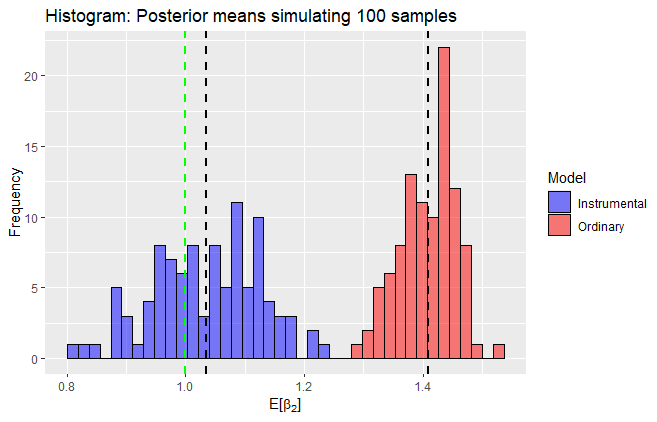
\includegraphics[width=340pt, height=200pt]{Chapters/chapter7/figures/Fig71.png}
	\caption[List of figure caption goes here]{Histogram of posterior means: Ordinary and instrumental models.}\label{fig71}
\end{figure}

Algorithm \ref{alg:IVReg} can be used to estimate the instrumental variable model using our GUI. We ask in Exercise 8 to replicate the example of the effect of institutions on per capita GDP using our GUI.  

\begin{algorithm}[h!]
	\caption{Instrumental variable model}\label{alg:IVReg}
	\begin{algorithmic}[1]  		 			
		\State Select \textit{Multivariate Models} on the top panel
		\State Select \textit{Variable instrumental (two equations)} model using the left radio button
		\State Upload the dataset selecting first if there is header in the file, and the kind of separator in the \textit{csv} file of the dataset (comma, semicolon, or tab). Then, use the \textit{Browse} button under the \textbf{Choose File} legend
		\State Select MCMC iterations, burn-in and thinning parameters using the \textit{Range sliders}
		\State Write down the formula of the structural equation in the \textbf{Main Equation} box. This formula must be written using the syntax of the \textit{formula} command of \textbf{R} software. This equation includes intercept by default, do not include it in the equation
		\State Write down the formula of the endogenous regressor in the \textbf{Instrumental Equation} box. This formula must be written using the syntax of the \textit{formula} command of \textbf{R} software. This equation includes intercept by default, do not include it in the equation
		\State Set the hyperparameters: mean vectors, covariance matrices, degrees of freedom, and the scale matrix. This step is not necessary as by default our GUI uses non-informative priors
		\State Click the \textit{Go!} button
		\State Analyze results
		\State Download posterior chains and diagnostic plots using the \textit{Download Posterior Chains} and \textit{Download Posterior Graphs} buttons
	\end{algorithmic} 
\end{algorithm}

\section{Multivariate probit model}\label{sec74}

In the multivariate probit model \cite{Edwards2003}, the response variable $y_{il}=\left\{0,1\right\}$ indicates that individual $i$ makes binary choices regarding no mutually exclusive alternatives $l$, $i=1,2,\dots,N$, $l=1,2,\dots,L$. In particular,
\begin{align*}
	y_{il}=\begin{Bmatrix}
		0, \ y_{il}^*\leq 0 \\ 
		1, \ y_{il}^*> 0 \\ 
	\end{Bmatrix},
\end{align*}
where $\bm{y}_{i}^*=\bm{X}_{i}\bm{\beta}+\bm{\mu}_{i}\stackrel{i.i.d.} {\thicksim}{N}(\bm0,\bm{\Sigma})$, $\bm{y}_i^*$ is an unobserved latent $L$-dimensional vector, $\bm{X}_{i}$ is an $L\times K$ design matrix of regressors, $K=L\times k$, $k$ is the number of regressors, and $\bm{\beta}=\left[\bm{\beta}_1^{\top} \ \bm{\beta}_2^{\top} \dots  \bm{\beta}_k^{\top}\right]^{\top}$, where the $\bm{\beta}_j$ make up an $L$-dimensional vector of coefficients, $j=1,2,\dots,k$. We simultaneously take into account the alternative-varying regressors (alternative attributes) and alternative-invariant regressors (individual characteristics).

The likelihood function in this model is $p(\bm{\beta},\bm{\Sigma}|\bm{y},\bm{X})=\prod_{i=1}^N\prod_{l=1}^L p_{il}^{y_{il}}$ where $p_{il}=p(y_{il}^*\geq 0)$.
Observe that $p({y}_{il}^*\geq 0)=p({\lambda}_{ll}{y}_{il}^*\geq 0)$, $\lambda_{ll}>0$. This generates identification issues because just the correlation matrix can be identified, same case as the univariate probit model where the variance of the model is fixed to 1. We follow the post processing strategy proposed by \cite{Edwards2003} to get identified parameters, that is, $\tilde{\bm{\beta}}=vec\left\{\bm{\Lambda}\bm{B}\right\}$ and the correlation matrix $\bm{R}=\bm{\Lambda}\bm{\Sigma}\bm{\Lambda}$, where $\bm{\Lambda}=diag\left\{\sigma_{ll}\right\}^{-1/2}$ and $\bm{B}=\left[\bm{\beta}_1,\bm{\beta}_2,\dots,\bm{\beta}_k\right]$.\footnote{In a Bayesian setting, we can have a non identified model; however, the posterior of the model parameters exists given a proper prior distribution \cite{Edwards2003}.}

We assume independent priors, $\bm{\beta}\sim{N}(\bm{\beta}_0,\bm{B}_0)$ and $\bm{\Sigma}^{-1}\sim{W}(\alpha_0,\bm{\Psi}_0)$.
We can employ Gibbs sampling in this model because this is a standard Bayesian linear regression model when data augmentation in $\bm{y}^*$ is used.
The posterior conditional distributions are

\begin{equation*}
	\bm{\beta}|\bm{\Sigma},\bm{w}\sim{N}(\bm{\beta}_n,\bm{B}_n),
\end{equation*}
\begin{equation*}
	\bm{\Sigma}^{-1}|\bm{\beta},\bm{w}\sim{W}(\alpha_n,\bm{\Psi}_n),
\end{equation*}
\begin{equation*}
	y_{il}^*|\bm{y}_{i,-l}^*,\bm{\beta},\bm{\Sigma}^{-1},\bm{y_i}\sim{T}{N}_{I_{il}}(m_{il},\tau_{ll}^2)
\end{equation*}

where $\bm{B}_n=(\bm{B}_0^{-1}+\bm{X}^{*\top}\bm{X}^*)^{-1}$, $\bm{\beta}_n=\bm{B}_n(\bm{B}_0^{-1}\bm{\beta}_0+\bm{X}^{*\top}\bm{y}^{**})$, $\bm{\Sigma}^{-1}=\bm{C}^{\top}\bm{C}$, $\bm{X}_i^{*\top}=\bm{C}^{\top}\bm{X}_i$, $\bm{y}_i^{**}=\bm{C}^{\top}\bm{y}_i^*$, $\bm{X}^*=\begin{bmatrix}\bm{X}_1^*\\
	\bm{X}_2^*\\
	\vdots\\
	\bm{X}_N^*
\end{bmatrix}$, $\alpha_n=\alpha_0+N$, $\bm{\Psi}_n=(\bm{\Psi}_0+\sum_{i=1}^N (\bm{y}_i^*-\bm{X}_i\bm{\beta})^{\top}(\bm{y}_i^*-\bm{X}_i\bm{\beta}))^{-1}$, $I_{il}=\begin{Bmatrix} y_{il}^*> 0, & y_{il}=1\\
	y_{il}^*\leq 0 , & y_{il}=0\\
\end{Bmatrix}$, $m_{il}=\bm{x}_{il}^{\top}\bm{\beta}+\bm{f}^{\top}(\bm{y}_{i,-l}^*-\bm{X}_{i,-l}\bm{\beta})$, $\bm{y}_{i,-l}^*$ is an $L-1$ dimensional vector of all components of $\bm{y}_i^*$ excluding $y_{il}^*$, $\bm{x}_{il}$ is the $l$-th row of $\bm{X}_i$, $\bm{X}_{i,-l}$ is $\bm{X}_{i}$ after deleting the $l$-th row, $\tau_{ll}^2=1/\sigma^{ll}$, and $\bm{f}=-\sigma^{ll}\bm{\omega}_{l,-l}$, $\sigma^{jl}$ is the $jl$-th element of $\bm{\Sigma}^{-1}$, $\bm{\Sigma}^{-1}=\begin{bmatrix}\bm{\omega}_1^{\top} \ \bm{\omega}_2^{\top} \vdots \bm{\omega}_{L}^{\top} \end{bmatrix}$, $\bm{\omega}_{l,-l}^{\top}$ is the $l$-th row of $\bm{\Sigma}^{-1}$ extracting the $l$-th element.\\


\textbf{Example: Self selection in hospitalization due to a subsidized health care program in Medell\'in}

We use the dataset \textit{7HealthMed.csv} where the dependent variable is equal to $y = \left[\text{Hosp} \ \text{SHI}\right]'$ where $\text{Hosp}$ is equal to 1 if an individual was hospitalized in 2007, 0 otherwise, and $\text{SHI}$ is equal to 1 if the individual had subsidized health insurance that year, and 0 otherwise.
Recall that our application in binary response models was to uncover the determinants of hospitalization in Medell\'in (Colombia), where one of the regressors was a binary indicator of being in a subsidized health care program.
We can use a bivariate probit model if we suspect there is a dependence regarding the decisions involving these two variables.
We would expect a priori that being in a subsidized health care program would imply a higher probability of being hospitalized \textit{ceteris paribus}.
However, if an individual expects to be hospitalized in the future, and the factors that drive this decision are unobserved to the econometrician, we would have a feedback effect from being hospitalized on being in a subsidized health care program.

We took into account 9 regressors: a constant, female, age, squared age, self perception of health status taking as reference bad (four categories), and the proportion of the individual's age spent living in her/his neighborhood (PTL). 
The last variable tries to take into account the social capital that can affect being in the subsidized health insurance program, as the target population is identified by the local government \cite{Ramirez2019a}. We have 12975 individuals chosen two options (subsidized regime and hospitalization).

The Algorithm \ref{alg:MtultProbit} shows how to run a multivariate probit model in our GUI. 

\begin{algorithm}[h!]
	\caption{Instrumental variable model}\label{alg:MtultProbit}
	\begin{algorithmic}[1]  		 			
		\State Select \textit{Multivariate Models} on the top panel
		\State Select \textit{Multivariate Probit} model using the left radio button
		\State Upload the dataset selecting first if there is header in the file, and the kind of separator in the \textit{csv} file of the dataset (comma, semicolon, or tab). Then, use the \textit{Browse} button under the \textbf{Choose File} legend
		\State Select MCMC iterations, burn-in and thinning parameters using the \textit{Range sliders}
		\State Write down the formula of the structural equation in the \textbf{Main Equation} box. This formula must be written using the syntax of the \textit{formula} command of \textbf{R} software. This equation includes intercept by default, do not include it in the equation
		\State Write down the formula of the endogenous regressor in the \textbf{Instrumental Equation} box. This formula must be written using the syntax of the \textit{formula} command of \textbf{R} software. This equation includes intercept by default, do not include it in the equation
		\State Set the hyperparameters: mean vectors, covariance matrices, degrees of freedom, and the scale matrix. This step is not necessary as by default our GUI uses non-informative priors
		\State Click the \textit{Go!} button
		\State Analyze results
		\State Download posterior chains and diagnostic plots using the \textit{Download Posterior Chains} and \textit{Download Posterior Graphs} buttons
	\end{algorithmic} 
\end{algorithm}


We set 20,000 MCMC iterations plus 1,000 iterations as burn-in, and a thinning parameter equal to 5.
This implies an effective length of the posterior chains equal to 4,000 draws.
We also used default values for the hyperparameters of the prior distributions.
In general, the convergence diagnostics seem good, except that there is a high level of autocorrelation for the posterior chain of the correlation between the two equations, as indicated by the dependence factors, and the trace and autocorrelation plots.
Observe that the tests of \cite{Geweke1992} and \cite{Heidelberger1983} have NaN values for the elements (1, 1) and (2, 2) of the covariance matrix, as these parameters were set equal to 1 due to identification restrictions.
This also means just two values for the dependence factors, which are actually the same due to symmetry.


\begin{tcolorbox}[enhanced,width=4.67in,center upper,
	fontupper=\large\bfseries,drop shadow southwest,sharp corners]
	\textit{R code. Self selection in hospitalization}
	\begin{VF}
		\begin{lstlisting}[language=R]
rm(list = ls()); set.seed(010101)
Data <- read.csv("DataApplications/7HealthMed.csv", sep = ",", header = TRUE, fileEncoding = "latin1")
attach(Data); str(Data)
p <- 2; nd <- 9; N <- length(y)/p; y <- y
Xd <- as.matrix(Data[seq(1, p*N, 2),3:11])
XcreateMP<-function(p,nxs,nind,Data){
	pandterm = function(message) {
		stop(message, call. = FALSE)
	}
	if (missing(nxs)) 
	pandterm("requires number of regressors: include intercept if required")
	if (missing(nind)) 
	pandterm("requires number of units (individuals)")
	if (missing(Data)) 
	pandterm("requires dataset")
	if (nrow(Data)!=nind*2)
	pandterm("check dataset! number of units times number alternatives should be equal to dataset rows")
	XXDat<-array(0,c(p,1+nxs,nind))
	XX<-array(0,c(p,nxs*p,nind))
	YY<-array(0,c(p,1,nind))
	is<- seq(p,nind*p,p)
	cis<- seq(nxs,nxs*p+1,nxs)
	for(i in is){
		j<-which(i==is)
		XXDat[,,j]<-as.matrix(Data[c((i-(p-1)):i),-1])
		YY[,,j]<-XXDat[,1,j]
		for(l in 1:p){
			XX[l,((cis[l]-(nxs-1)):cis[l]),j]<-XXDat[l,-1,j]
		}
	}
	return(list(y=YY,X=XX))
}
Dat <- XcreateMP(p = p, nxs = nd, nind = N, Data = Data)
y<-NULL; X<-NULL
for(i in 1:dim(Dat$y)[3]){
	y<-c(y,Dat$y[,,i])
	X<-rbind(X,Dat$X[,,i])
}
DataMP = list(p=p, y=y, X=X)
# Hyperparameters
k <- dim(X)[2]; b0 <- rep(0, k); c0 <- 1000; B0 <- c0*diag(k)
B0i <- solve(B0); a0 <- p - 1 + 3; Psi0 <- a0*diag(p)
Prior <- list(betabar = b0, A = B0i, nu = a0, V = Psi0)
# MCMC parameters
mcmc <- 100000; thin <- 5
Mcmc <- list(R = mcmc, keep = thin)
\end{lstlisting}
	\end{VF}
\end{tcolorbox}

\begin{tcolorbox}[enhanced,width=4.67in,center upper,
	fontupper=\large\bfseries,drop shadow southwest,sharp corners]
	\textit{R code. Self selection in hospitalization, results}
	\begin{VF}
		\begin{lstlisting}[language=R]
Results <- bayesm::rmvpGibbs(Data = DataMP, Mcmc = Mcmc, Prior = Prior)
betatilde <- Results$betadraw / sqrt(Results$sigmadraw[,1])
attributes(betatilde)$class <- "bayesm.mat"
summary(coda::mcmc(betatilde))
Quantiles for each variable:
2.5%        25%        50%        75%     97.5%
var1  -5.5137018 -1.946e+00 -1.298e+00 -6.494e-01 2.9004506
var2   0.0327632  9.315e-02  1.252e-01  1.572e-01 0.2178014
var3  -0.0078208 -3.120e-03 -6.648e-04  1.798e-03 0.0065977
var4  -0.0000417  1.462e-05  4.411e-05  7.356e-05 0.0001297
var5  -3.8462383 -2.747e-01  3.677e-01  1.015e+00 4.5937307
var6  -4.3469133 -7.901e-01 -1.459e-01  4.952e-01 4.0485322
var7  -5.0522003 -1.496e+00 -8.543e-01 -2.101e-01 3.3375816
var8  -4.9152373 -1.360e+00 -7.058e-01 -7.392e-02 3.4898306
var9  -0.1838265 -1.097e-01 -6.940e-02 -2.936e-02 0.0472931
var10 -2.8060844  3.396e-01  1.169e+00  2.732e+00 6.3954827
var11  0.2280206  5.567e-01  9.842e-01  2.293e+00 3.3507157
var12 -0.0574587 -2.311e-02 -9.777e-03 -3.976e-03 0.0033351
var13  0.0001256  3.125e-04  5.964e-04  1.323e-03 0.0020878
var14 -3.0896704  2.245e-01  9.712e-01  2.419e+00 6.1875147
var15 -3.8584533 -1.963e-01  3.769e-01  1.285e+00 4.8754045
var16 -4.5826124 -8.322e-01 -1.249e-01  4.637e-01 3.9548010
var17 -4.5922641 -9.026e-01 -1.634e-01  4.225e-01 3.9128193
var18  0.1511020  3.760e-01  7.023e-01  1.561e+00 2.4146495
sigmadraw <-  Results$sigmadraw / Results$sigmadraw[,1]
attributes(sigmadraw)$class = "bayesm.var"
summary(coda::mcmc(sigmadraw))
Quantiles for each variable:
2.5%     25%       50%      75%    97.5%
var1  1.0000  1.0000  1.000000  1.00000   1.0000
var2 -0.4574 -0.0828 -0.007985  0.05506   0.3883
var3 -0.4574 -0.0828 -0.007985  0.05506   0.3883
var4  0.5711  3.3214  9.789460 56.30992 110.2846
\end{lstlisting}
	\end{VF}
\end{tcolorbox}


The results suggest that only female is relevant to explain hospitalization.
The 95\% credible interval is (3.13e-02, 0.22).
Observe that only 3.11\% of the sample has been hospitalized.
Probit models are not well designed for this kind of dataset, but our main purpose is to illustrate the use of our GUI.
On the other hand, the results suggest that age, squared age, and the proportion of age spent living in the neighborhood are statistically relevant to explain enrollment in the subsidized program.
Their 95\% credible intervals are (2.63e-01, 3.27e-01), (-8.05e-03, -2.05e-03) and (0.15, 0.27), respectively.
The latter result seems to support the social capital hypothesis.
Lastly, the 95\% credible interval for the correlation between the two binary equations is (-0.07, 0.06), suggesting that there is no self selection regarding these two decisions (hospitalization and subsidized insurance).
So, it seems that it is better to estimate univariate binary models for each of these dependent variables, for the sake of parsimony.



\section{Summary}\label{sec75}

\section{Exercises}\label{sec76}
\begin{enumerate}
	\item Show that $\mathbb{E}[u_1\text{PAER}]=\frac{\alpha_1}{1-\beta_1\alpha_1}\sigma^2_1$ assuming that $\mathbb{E}[u_1u_2]=0$ where $Var(u_1)=\sigma^2_1$ in the effect of institutions on per capita GDP.
	
	\item Show that $\beta_1=\pi_1/\gamma_1$ in the effect of institutions on per capita GDP.
	
	\item \textbf{The effect of institutions on per capita gross domestic product continues I}
	
	Use the \textit{rmultireg} command from the \textit{bayesm} package to perform inference in the example of the effect of institutions on per capita GDP. 
	
	\item \textbf{Demand and supply simulation}
	
	Given the structural demand-supply model:
	\begin{align*}
		q_i^d&=\beta_1+\beta_2p_i+\beta_3y_i+\beta_4pc_i+\beta_5ps_i+u_{i1}\\
		q_i^s&=\alpha_1+\alpha_2p_i+\alpha_3er_i+u_{i2},
	\end{align*}
where $q^d$ is demand, $q^s$ is supply, $p$, $y$, $pc$, $ps$ and $er$ are price, income, complementary price, substitute price, and exchange rate. Complementary and substitute prices are prices of a complementary and substitute goods of $q$. Assume that $\bm{\beta}=\left[5 \ -0.5 \ 0.8 \ -0.4 \ 0.7\right]^{\top}$, $\bm{\alpha}=\left[-2 \ 0.5 \ -0.4\right]^{\top}$, $u_1\sim N(0, 0.5^2)$ and $u_2\sim N(0, 0.5^2)$. In addition, assume that $y\sim N(10,1)$, $pc\sim N(5,1)$, $ps\sim N(5,1)$ and $tc\sim N(15,1)$.
\begin{itemize}
	\item Find the \textit{reduce-form} model using that in equilibrium demand and supply are equal, that is, $q^d=q^s$. This condition defines the observable quantity ($q$).
	\item Simulate $p$ and $q$ from the \textit{reduce-form} equations.
	\item Preform inference of the \textit{reduce-form} model using the \textit{rmultireg} command from the \textit{bayesm} package.
	\item Use the posterior draws of the \textit{reduce-form} parameters to perform inference of the \textit{structural} parameters. Any issue? Hint: Are all \textit{structural} parameters exactly identified?   
\end{itemize}

\item \textbf{Utility demand continues}

\begin{itemize}
	\item Run the \textbf{Utility demand} application using our GUI and the information in the dataset \textit{Utilities.csv}. Hint: This file should be modified to agree the structure that requires our GUI (see the dataset \textit{5Institutions.csv} in the folder \textit{DataApp} of our GitHub repository -\textbf{https://github.com/besmarter/BSTApp}- for a template).
	\item Program from scratch the Gibbs sampler algorithm in this application.   
\end{itemize}

\item \textbf{Simulation exercise of instrumental variables continues I}

\begin{enumerate}
	\item Use the setting of the simulation exercise of instrumental variables to analyze what happens when the instrument is weak, for instance, setting $\gamma_2=0.2$, and compare the performance of the posterior means of the ordinary and instrumental models.
	\item Perform a simulation that helps to analyze how the degree of exogeneity of the instrument affects the performance of the posterior mean of the instrumental variable model.	 
\end{enumerate}

\item \textbf{Simulation exercise of instrumental variables continues II}

Program from scratch the Gibbs sampling algorithm of the instrumental model for the simulation exercise of the instrumental variables.

\item \textbf{The effect of institutions on per capita gross domestic product continues II}

Estimate the structural Equation \ref{eq:str1} using the instrumental variable model where the instrument of PAER is $\log(\textit{Mort})$. Compare the effect of property rights on per capita GDP of this model with the effect estimated in the example of the effect of institutions on per capita gross domestic product. Use the file \textit{6Institutions.csv} to do this exercise in our GUI, and set $\bm{B}_0=100\bm{I}_5$, $\bm{\beta}_0=\bm{0}_5$, $\bm{\gamma}_0=\bm{0}_2$, $\bm{G}_0=100\bm{I}_2$ $\alpha_0=3$ and $\bm{\Psi}_0=3\bm{I}_2$. The MCMC iterations, burn-in and thinning parameters are 50000, 1000 and 5, respectively. 

\end{enumerate}


